\documentclass[12pt,t]{beamer}
\usepackage{graphicx}
\usepackage[vlined]{algorithm2e}
\usepackage{times}
\usepackage{calc}
\usepackage{url}
\usepackage{soul}
\usepackage{graphicx}
\usepackage{multirow, hhline}
\usepackage{array, booktabs}
\usepackage{amsmath}
\usepackage{amssymb}
\usepackage{relsize}
\usepackage{multirow}
\usepackage{booktabs}
\usepackage{pagecolor}
\usepackage{lipsum}
\usepackage{capt-of}
\usepackage{booktabs}

\usepackage{graphicx}
\usepackage{multicol}
\usepackage[T1]{fontenc}
\usepackage{ae}
\graphicspath{{fig/}}
\setbeameroption{hide notes}
\setbeamertemplate{note page}[plain]

\usetheme{default}
\beamertemplatenavigationsymbolsempty
\hypersetup{pdfpagemode=UseNone}

\usefonttheme{professionalfonts}
\usefonttheme{serif}
\usepackage{fontspec}
\setmainfont{Karla}
\setbeamerfont{note page}{family*=pplx,size=\footnotesize} % Palatino for notes

\definecolor{foreground}{RGB}{70,70,70}
\definecolor{background}{RGB}{249, 249, 249} %24,24,24
%\definecolor{title}{RGB}{107,174,214} %107,174,214
\definecolor{title}{RGB}{70,70,70}
\definecolor{gray}{RGB}{0,0,0}
\definecolor{subtitle}{RGB}{70,70,70}
\definecolor{hilight}{RGB}{102,255,204}
\definecolor{vhilight}{RGB}{255,111,207}

\setbeamercolor{titlelike}{fg=title}
\setbeamercolor{subtitle}{fg=subtitle}
\setbeamercolor{institute}{fg=gray}
\setbeamercolor{normal text}{fg=foreground,bg=background}


\setbeamercolor{item}{fg=foreground} % color of bullets
\setbeamercolor{subitem}{fg=gray}
\setbeamercolor{itemize/enumerate subbody}{fg=gray}
\setbeamertemplate{itemize subitem}{{\textendash}}
\setbeamerfont{itemize/enumerate subbody}{size=\footnotesize}
\setbeamerfont{itemize/enumerate subitem}{size=\footnotesize}

\setbeamercolor{block title}{fg=white,bg=gray!70}
\setbeamercolor{block body}{fg=black,bg=gray!10}
\setbeamercolor{block title alerted}{fg=red,bg=gray!40}
\setbeamercolor{block title example}{fg=black,bg=green!20}
\setbeamercolor{block body example}{fg=black,bg=green!5}
\setbeamerfont{block title}{series=\bfseries}

\hypersetup{colorlinks,linkcolor=foreground,urlcolor=foreground}


\setbeamertemplate{footline}{%
    \raisebox{5pt}{\makebox[\paperwidth]{\hfill\makebox[20pt]{\color{gray}
          \scriptsize\insertframenumber}}}\hspace*{5pt}}

\addtobeamertemplate{note page}{\setlength{\parskip}{12pt}}


\newcommand{\bi}{\begin{itemize}}
\newcommand{\ei}{\end{itemize}}
\newcommand{\ig}{\includegraphics}
\newcommand{\subt}[1]{{\footnotesize \color{subtitle} {#1}}}

\let\emph\relax % there's no \RedeclareTextFontCommand
\DeclareTextFontCommand{\emph}{\bfseries\em}


\setbeamertemplate{frametitle}
{\vskip4pt
  \leavevmode
%\hbox{%
\begin{beamercolorbox}[wd=\paperwidth,ht=2ex,dp=0ex]{frametitle}%
\underline{\makebox[\paperwidth][l]{\hspace*{10pt}
\large {{\insertframetitle}}}}
\end{beamercolorbox}
%  }%
}

%\setbeamercolor{frametitle}{fg=yellow,bg=red}

\begin{document}

\AtBeginSection[]{
  \begin{frame}
  \vfill
  \centering
  \begin{beamercolorbox}[sep=8pt,center,shadow=true,rounded=true]{title}
    \underline{\makebox[0.6\paperwidth][l]{
\large {{\insertsectionhead}}}}
  \end{beamercolorbox}
  \vfill
  \end{frame}
}

\title{\large{Lecture \#17: Stacking}}
\subtitle{CS 109A, STAT 121A, AC 209A: Data Science}
\author{Pavlos Protopapas \and Kevin Rader}
%\institute{Harvard University}
\date{}
\titlegraphic{
   
\includegraphics[height=2cm]{iacs}
\includegraphics[height=2cm]{hogwarts}
}
{
\setbeamertemplate{footline}{} % no page number here
\frame{
  \titlepage
  
}
}


\begin{frame}{Lecture Outline}
\tableofcontents
\end{frame}

%%%%%%%%%%%%%%%%%%%%%%%%%%%%%%%%%%%%%%%%%%%%%%%%%%%%%%%%%%%%%%%%%%%%%%%%%%%%%%
\section{Review}

%%%%%%%%%%%%%%
\begin{frame}{Review of Ensemble Methods} 
\vskip-0.4cm
So far we've seen a variety of ensemble methods:
\only<1>{
\vskip0.2cm
\begin{itemize}
\item \textbf{Bagging}
\begin{itemize}
\item simultaneous training using bootstrap samples of data but the same set of predictors
\vskip0.1cm
\item ensemble is averaged to produce final model
\end{itemize}
\vskip0.2cm
\item \textbf{Random Forest}
\begin{itemize}
\item simultaneous training using bootstrap samples of data
\vskip0.1cm
\item models trained on random samples of predictors
\vskip0.1cm
\item  ensemble is averaged to produce final model
\end{itemize}
\vskip0.2cm
\item \textbf{Boosting} 
\begin{itemize}
\item serial training using common set of data and predictors
\vskip0.1cm
\item each new model is trained focusing on regions of error in the previous model
\vskip0.1cm
\item ensemble is summed to produce the final model
\end{itemize}
\end{itemize}
}

\only<2>{
\begin{itemize}
\item \textbf{Bagging  and Random Forest}
\vskip0.1cm
\begin{itemize}
\item low bias - ensemble of complex models 
\vskip0.1cm
\item low variance - variance is reduced via averaging and de-correlating models in ensemble
\end{itemize}
\item \textbf{Boosting}
\vskip0.1cm
\begin{itemize}
\item low bias - training error iteratively reduced
\vskip0.1cm
\item low variance - ensemble of simple models
\end{itemize}
\end{itemize}
}
\end{frame}





%%%%%%%%%%%%%%%%%%%%%%%%%%%%%%%%%%%%%%%%%%%%%%%%%%%%%%%%%%%%%%%%%%%%%%%%%%%%%%
\section{Stacking}

%%%%%%%%%%%%%%
\begin{frame}{Motivation for Stacking} 

Recall that in boosting, the final model $T$, we learn is a weighted sum of simple models, $T_h$,
\[
T = \sum_h \lambda_h T_h.
\]
where $\lambda_h$ is the learning rate. In AdaBoost for example, we can analytically determine the optimal values of $\lambda_h$ for each simple model $T_h$. 
\vskip0.2cm
On the other hand, we can also determine the final model $T$ implicitly by \emph{learning any  model, called meta-learner, that transforms the outputs of $T_h$ into a prediction}.

\end{frame}


%%%%%%%%%%%%%%
\begin{frame}{Stacked Generalization} 
\only<1>{
The framework for \emph{stacked generalization} or \emph{stacking} (Wolpert 1992) is:
\vskip0.2cm
\begin{itemize}
\item train $L$ number of models, $T_l$ on the training data
\[
\{(x_1, y_1), \ldots, (x_N, y_N) \}
\]
\vskip0.2cm
\item train a meta-learner $\widetilde{T}$ on the predictions of the ensemble of models, i.e. train using the data
\[
\{(T_1(x_1), \ldots, T_L(x_1), y_1), \ldots, (T_1(x_N), \ldots, T_L(x_N), y_N)\}
\]
\end{itemize}
}
\only<2>{
\begin{center}
\vskip-0.4cm
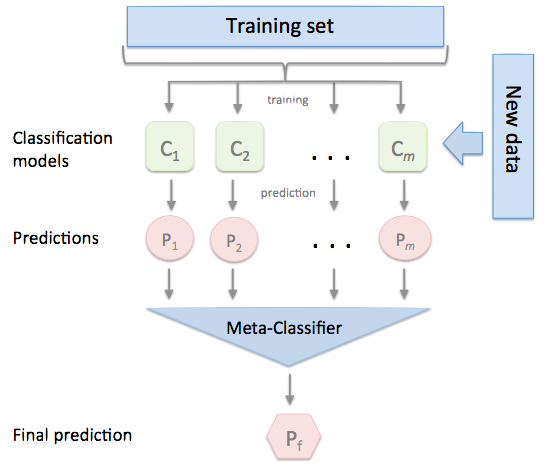
\includegraphics[width=90mm]{lecture17_g1.png}
\end{center}
}

\only<3>{
\vskip-0.4cm
Stacking is a very general method,
\vskip0.2cm
\begin{itemize}
\item the models, $T_l$, in the ensemble can come from different classes. The ensemble can contain a mixture of logistic regression models, trees etc.
\vskip0.2cm
\item the meta-learner, $T$, can be of any type. 
\end{itemize}
\vskip0.2cm
\textbf{Note:} we want to train $T$ on the \emph{out of sample} predictions of the ensemble. For example we train $T$ on 
\[
\{(T_1(x_1), \ldots, T_L(x_1), y_1), \ldots, (T_1(x_N), \ldots, T_L(x_N), y_N)\}
\]
where $T_l(x_n)$ is generated by training $T_l$ on 
\[
\{ (x_1, y_1), \ldots, (x_{n-1}, y_{n-1}), (x_{n+1}, y_{n+1}), \ldots, (x_N, y_N)\}.
\]
}
\end{frame}

%%%%%%%%%%%%%%
\begin{frame}{Stacking: General Guidelines} 
\vskip-0.4cm
The flexibility of stacking makes it widely applicable but difficult to analyze theoretically. Some general rules have been found through empirical studies:
\vskip0.2cm
\begin{itemize}
\item models in the ensemble should be diverse, i.e. their errors should be be uncorrelated
\vskip0.2cm
\item for classification, each model in the ensemble should have error rate < 1/2
\vskip0.2cm
\item if models in the ensemble outputs probabilities, it's better to train the meta-learner on probabilities rather than predictions
\vskip0.2cm
\item apply regularization to the meta-learner to avoid overfitting
\end{itemize}
\end{frame}

%%%%%%%%%%%%%%
\begin{frame}{Stacking: Subsemble Approach} 
\vskip-0.4cm
We can extend the stacking framework to include ensembles of models that specialize on small subsets of data (Sapp et. al. 2014), for de-correlation or improved computational efficiency:
\vskip0.2cm
\begin{itemize}
\item divide the data in to $J$ subsets
\item train a models , $T_j$, on each subset
\vskip0.2cm
\item train a meta-learner $\widetilde{T}$ on the predictions of the ensemble of models, i.e. train using the data
\[
\{(T_1(x_1), \ldots, T_J(x_1), y_1), \ldots, (T_1(x_N), \ldots, T_LJ(x_N), y_N)\}
\]
\end{itemize}
\vskip0.2cm
Again, we want to make sure that each $T_j(x_n)$ is an out of sample prediction. 
\end{frame}

%%%%%%%%%%%%%%
\begin{frame}{Example: Comparison of Ensemble Methods} 

\end{frame}
\end{document}
